\chapter{Introduction}

\epigraph{
  Race de Caïn, au ciel monte,\\
  Et sur la terre jette Dieu !
}{---\textcite[16]{baudelaire-1857}}


Category theory is a branch of mathematics developed in the 1940s
which has come to occupy a central position in computer science.


``Category theory is a relatively young branch of pure mathematics,
stemming from an area---algebraic topology---that most computer
scientists would consider esoteric. Yet its influence is being felt in
many parts of computer science, including the design of functional and
imperative programming languages, implementation techniques for
functional languages, semantic models of programming languages, models
of concurrency, type theory, polymorphism, specification languages,
constructive logic, automata theory, and the development of
algorithms'' \parencite[xi]{pierce-1991}.


``Developed in the 1940s as a way to organize constructs in algebraic
topology, category theory works at a level of whole mathematical
objects rather than their elements. (...) Category theory can be
viewed as a formalization of operations on abstract data types in
computer languages'' \parencite[1154]{wolfram-2002}.

``Category theory has come to occupy a central position in
contemporary mathematicas and theoretical computer science. Roughly,
it s a general mathematical theory of structures and of systems of
structures. As CT is still evolving, its functions are correspondingly
developing, expandind and multiplying'' \parencite[1]{marquis-2013}.
``Category theory thus affords philosophers and logicians much to use
and reflect upon'' \parencite[1]{marquis-2013}. ``From the 1980s to
the present, category theory has found new applications. In
theoretical computer science, category theory is now firmly rooted,
and contributes, among other things, to the development of new logical
systems and to the semantics of programming''
\parencite[23]{marquis-2013}.








``One does not so much learn category theory as absorb it over a
period of time'' \parencite[26]{bird-demoor-1997}.

\todo{When speaking of Haskell, we refer to GHC. Important, for
  instance, when mentioning language options such as
  \texttt{KindSignatures}. We refer to GHC 7.4.2 and the Haskell
  platform 2012.4.0.0. We refer to Agda 2.3.2 and the Agda standard
  library 0.7.}

\todo{Prerequisite: Haskell or some of the concepts in a functional
  programming language (Functors, monads, polymorphic functions,
  etcetera) and Agda. Refer to tutorials.}

\todo{How about assuming something like the following:}
\begin{codehaskell}
import Prelude ()
\end{codehaskell}

\todo{Mention Abel. I deleted that chapter.}

``The trinity of concepts category, functor, and natural
transformation is what category theory is built on''
\parencite{nlab-category-theory}.

\section*{Summary of the project proposal}

This is an undergraduate project submitted in partial fulfillment of
the requirements for the degree of Systems Engineering at EAFIT. Here
is a summary of the project proposal, submitted in November 14, 2010.

\paragraph{Theoretical framework and proposal}

Category theory is a relatively recent branch of mathematics which
occupies a central position en contemporary mathematics and
theoretical computer science. The object of study of category theory
are known as categories. Basically, a category is an aggregate of
objects and mappings (morphisms or arrows) between objects. The most
known example is the category Set, the category of sets and functions.
The definition of category is important to present some notions (such
as functors and natural transformations) which make category theory a
common tool which organizes and unifies many aspects of mathematics.
(Marquis 2010)

Some functional programming languages (such as Haskell) have certain
important concepts for relating category theory to programming. In
this sense, polymorphism, algebraic data types, and the functor and
monad type classes, etc., are concepts which can be conceptualized or
are based on ideas from category theory. Even if its categorical
conceptualization is not necessary for its use, it's an ideal
complement for better understanding functional programming and its
theoretical foundations. (Haskell community)

Having this into account (that it is possible to conceptualize many
concepts of functional programming via the study of category theory,
this project aims to develop a monographical study of category theory
which allows to describe and explain some of the applications to
functional programming. In particlar, ...

Polymorphism refers to the fact that the type of a value may depend on
the context in which it is used. Algebraic data types have various
alternatives or constructors of values. Type classes allow to define
generic interfaces which exhibit characteristics common to a great
variety of types. Finally, a functor (in Haskell) is a class of types
which can be mapped and a monad (of Haskell) is a class of types which
introduces the concepts of context and the use of normal functions
which preserve the contexts of those contexts. (Real World Haskell).


\paragraph{Objective}

Our goal is to describe and explain some of the applications of
category theory to functional programming. More specifically, to
describe and explain the concepts of category theory which allow to
conceptualize and better understand the following concepts of
functional programming: polymorphism, algebraic data types, and the
functor and monad type classes.

\paragraph{Justification}

The study of category theory allows to deepen scientific knowledge and
discover some of its practical applications to subjects that the
author has identified as important and interesting for his Systems
Engineering.

This project allows to study a topic related with computer science and
to deepen the study of theoretical foundations of the undergraduate.

The study of category theory will allow to understand and apply
effectively and efficiently the theoretical foundations of functional
programming. Category theory is a solid framework for a lot of
concepts of functional programming.

Even though the study of theoretical foundations of functional
programming is not strictly necessary for a programmer, it is an ideal
complement for his appropriate education and adequate understanding of
the theoretical and practical concepts of programming.

Category theory is a common tool which organizes and unifies many
aspects of mathematicals, which makes it an important tool for
studying the theoretical foundations of functional programming.

Category theory arises naturally in many areas of computer science and
programming (language design, formal semantics, type systems, et
cetera) (Hutton 2010), which makes it an important tool for studying
the foundations of some programming areas.

Even though the categorical formulation of some concepts may be
difficult to understand, category theory is a conceptual framework
which allows to deal with such concepts at a higher level of
abstraction.

\paragraph{Methodology}

The methodology used for the development of this project consists of
four stages: researching, reading, writing, and revision

\paragraph{Scope}

This study of category theory is restricted to the following concepts:

\begin{enumerate}
\item Introductory concepts and infrastructure of category theory
  \begin{enumerate}
  \item Categories
  \item Infrastructure of category theory
    \begin{itemize}
    \item Monomorphisms, epimorphisms, and isomorphisms
    \item Initial and terminal objects
    \item Universal constructions
    \end{itemize}
  \end{enumerate}
\item Basic concepts of category theory
  \begin{enumerate}
  \item Functors
  \item Natural transformations
  \item Adjunctions
  \item Limits
  \end{enumerate}
\item More specific concepts of category theory
  \begin{enumerate}
  \item Algebras
  \item Monads
  \end{enumerate}
\end{enumerate}

\paragraph{Product or result}

The result of this project is a monograph on category theory and some
of its applications to functional programming. This monograph contains
the results of the development of the project, that is, the results of
the writing stage.

\paragraph{Audience}

The main audience of this project is any computer scientist with an
interest in mathematicas, the theoretical foundations of computer
science or functional programming.

\section*{Overview of the project}

The project is divided into six chapters.

\todo{This work (undergraduate dissertation or thesis or project?) is
  divided into six chapters. The chapters are more or less dependent
  on each other, but there are two lines.} See Figure \ref{fig:overview}.

Chapter \ref{chap:categories} is about categories. Required for all
chapters. Including a category for Haskell and a category for Agda.

Chapter \ref{chap:constructions} describes constructions. This chapter
is essential background for Chapter \ref{chap:algebras}, less
important for Chapter \ref{chap:functors}, and not so necessary for
the rest. Such as isomorphisms, initial and terminal objects, products
and coproducts. Includes examples in \set, in Haskell, and Agda.

Chapter \ref{chap:functors} studies functors. Mathematical, in Haskell
and Agda.

Chapter \ref{chap:naturals} describes natural transformations. And
natural transformations or polymorphic functions in Haskell.

Chapter \ref{chap:monads} is about monads. And Kleisli triples. And in
Haskell and Agda.

Chapter \ref{chap:algebras} is about algebras over endofunctors. Just
in Haskell.

Additionally, in Chapter \ref{chap:conclusions}, we

Each chapter... \todo{Each chapter has a similar structure. A
  motivation, theory, and Haskell. Some chapters include an analysis
  in Agda. Each chapter ends with a References section, which collects
  historical comments, and references to the literature. A reference
  is a mention or citation of a source of information. Each chapter
  should have references to books covering the subject in greater
  depth. Each chapter is referenced.}

Finally, in Appendix \ref{chap:references}, we...

\begin{figure}[htb]
  \begin{center}
    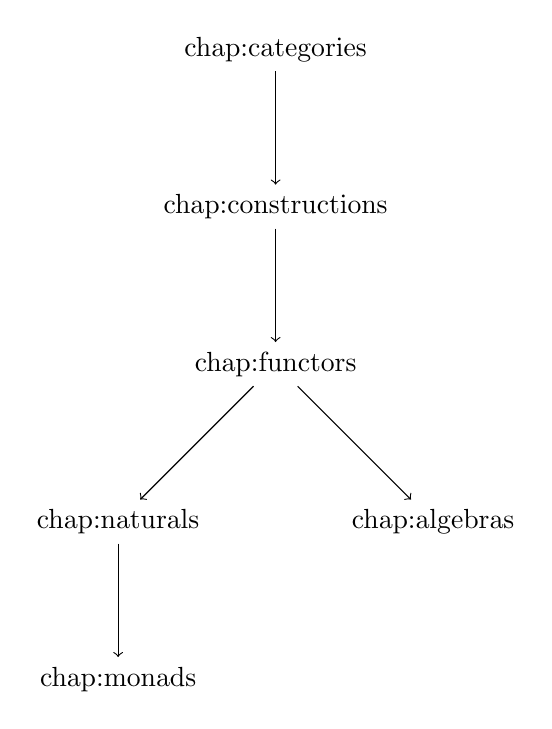
\begin{tikzpicture}
      \node (categories)    at (2,8) {\nameref{chap:categories}};
      \node (constructions) at (2,6) {\nameref{chap:constructions}};
      \node (functors)      at (2,4) {\nameref{chap:functors}};
      \node (naturals)      at (0,2) {\nameref{chap:naturals}};
      \node (monads)        at (0,0) {\nameref{chap:monads}};
      \node (algebras)      at (4,2) {\nameref{chap:algebras}};

      \draw [->] (categories)    to (constructions);
      \draw [->] (constructions) to (functors);

      \draw [->] (functors)      to (naturals);
      \draw [->] (naturals)      to (monads);

      \draw [->] (functors)      to (algebras);

    \end{tikzpicture}
  \end{center}
  \caption{Overview of the project.}
  \label{fig:overview}
\end{figure}

\subsection*{Links}

And Abel in
\begin{center}
  \url{https://github.com/jpvillaisaza/abel}
\end{center}

\clearemptydoublepage
